% HSPMN v5: final arXiv paper.
% Single-voice rewrite, 2026-06-10. All numbers verified against results/ and
% terminal checkpoints (commit cb37971 audit). Theorem inlined (Pinsker form).
% Style: no em dashes; plain declarative prose; figures + honest limitations.

\documentclass[11pt,a4paper]{article}
\usepackage[utf8]{inputenc}
\usepackage{amsmath, amssymb, amsthm}
\usepackage{graphicx}
\usepackage{booktabs}
\usepackage{xcolor}
\usepackage[numbers]{natbib}
\usepackage[colorlinks=true,citecolor=blue,linkcolor=blue]{hyperref}
\usepackage{geometry}
\usepackage{microtype}
\geometry{margin=1in}

\newtheorem{proposition}{Proposition}
\newtheorem{corollary}{Corollary}
\newcommand{\LL}{\mathcal{L}}
\newcommand{\EE}{\mathbb{E}}
\newcommand{\norm}[1]{\left\lVert#1\right\rVert}

\title{Nothing to Route On: A Measured Information Ceiling Explains\\
Routing Absorption in Hybrid Mamba-Attention Language Models}
\author{Szymon J\k{e}dryczko \\
Tenzan Logic, Krak\'ow}
\date{June 2026}

\begin{document}
\maketitle

\begin{abstract}
Small hybrid language models pair an attention stream with a state-space
stream and add a learned gate that decides, token by token, how much each
stream contributes. We ask a simple question: does the gate actually do
anything? Across 134 training runs at 140M and 350M parameters on a single
consumer GPU, the answer is no, and we can measure why.

First, the architecture. A block-level dual-stream design with a learned
router loses to plain head-level fusion by $+19.5\%$ perplexity at matched
parameters and ingredients. The loss traces to the router itself: on the
trained checkpoint, 6 of 12 layers gate every token to zero and two more
route under $0.03\%$ of tokens. Second, the gate. With the router removed
and a per-token sigmoid gate added back in its simplest form, the learned
gate fails to beat a frozen random gate at 140M and again at 350M (3 seeds
each), reproducing the routing-absorption result of Aquino-Michaels at
$11\times$ their scale.

Third, the explanation. We treat the gate as a noisy channel between the
token and the event ``the attention stream lowers the loss here,'' and
prove via Fano and Pinsker inequalities that a gate's benefit over an
always-on baseline is capped by $\sqrt{2(I + \log 2 - H(s))}$, where $I$
is the mutual information the gate carries about that event and $H(s)$
the event's entropy. Full routing
benefit needs about $0.72$ bits. Trained gates carry $0.004$ to $0.006$
bits. An optimal probe, trained directly on the oracle label with access
to both streams' outputs, reaches at most $0.037$ bits: twenty times
short. The routing target is nearly information-free, so no token-local
gate of this class can work, trained or not. A final probe shows why:
ablating the attention stream hurts on 256 of 256 held-out sequences, and
$98.9\%$ of the benefit variance lies within sequences. The optimal
routing policy is ``always on,'' which is the gate-less baseline. The
gates fail not because routing is hard to learn but because, on this
data, there is nothing to route on.

Finally, the way out. The theory leaves two levers, data heterogeneity
and stream non-redundancy, and we test both in a pre-registered
programme. Dialling recall-heavy segments into the corpus raises the
measured ceiling $7.9\times$, as predicted, while every perplexity null
lands where the bound puts it; a stream-decorrelation regulariser fails
to move the ceiling, closing the simplest architecture lever.

All experiments run on one NVIDIA RTX 5090. Code, checkpoint logs, and
per-seed numbers accompany the paper.
\end{abstract}

\section{Introduction}
\label{sec:intro}

Hybrid language models are built on an attractive bargain. Attention is
precise but expensive; state-space recurrences such as Mamba are cheap but
lossy on recall. So the field combines them, and almost every combination
ships a routing mechanism: a learned gate, a router, a per-token mixture
weight that decides which stream handles which token
\citep{hymba,jamba,mor}. The implicit promise is that tokens differ, that
some need attention and some do not, and that a learned gate can tell them
apart.

\citet{absorption2026} tested that promise at 31M parameters and found it
empty: a model with a learned gate reached the same perplexity as the same
model with a frozen random gate ($48.73 \pm 0.60$ vs $49.83 \pm 0.04$).
They named the failure \emph{routing absorption}: the trainable network
around the gate compensates for whatever the gate does, so the gate adds
nothing. Their result is empirical and small-scale, and it left two open
questions. Does absorption persist at larger scale and across architecture
families? And is it a contingent training failure, something a better gate
or a better optimiser would fix, or a structural property of the problem?

This paper answers both questions, the second one quantitatively. We run
the comparison the absorption literature has been missing: matched
parameters, matched ingredients, multiple seeds, two scales, on a fixed
public corpus, with the random-gate control that \citet{absorption2026}
made mandatory. We then go past the null result and measure the
information that any gate of this class could possibly use, which turns
the null into an impossibility with a number attached.

We make five contributions.

\textbf{1. Block fusion retired, with a mechanism (\S\ref{sec:exp-140m},
\S\ref{sec:h1}).} At 140M parameters on wikitext-103, with 3 seeds and a
per-variant learning-rate sweep, a block-level dual-stream design with a
ReLU router (in the style of our earlier HSPMN v4, using Native Sparse
Attention \citep{nsa} and Gated DeltaNet \citep{gateddeltanet}) loses to head-level fusion of the same two ingredients by
$+19.5\%$ perplexity, while also costing $19\%$ more forward FLOPs per
token. The cause is visible in the trained weights: the router collapses
modally. Six of twelve layers gate every token to zero, two more are
effectively dead (under $0.03\%$ of tokens routed), two layers
saturate (one with gate magnitudes near 47 and a standard deviation of
316), and the load balancer hides this by averaging healthy-looking
statistics across layers. Head fusion, which mixes streams structurally
inside the projection and has no router to collapse, simply works:
$139.14 \pm 8.43$ perplexity against a $\mu$P-tuned dense baseline's
$144.01 \pm 5.64$.

\textbf{2. The gate null, replicated at two scales
(\S\ref{sec:exp-140m}, \S\ref{sec:exp-350m}).} On the head-fusion
architecture we then ablate the gate question directly: gate-less, learned
per-token sigmoid gate, frozen random gate (the Aquino-Michaels control),
and a parameter-free content gate. At 140M the learned gate is
indistinguishable from random ($143.85 \pm 9.27$ vs $146.24 \pm 7.56$) and
both lose to no gate at all ($139.14 \pm 8.43$). At 350M, with 3 seeds
each, the same: $82.35 \pm 4.78$ vs $83.79 \pm 1.37$, Welch
$t \approx -0.41$. A seed-42 run that initially looked like a $10\%$ win
for the learned gate turned out to be seed luck; the same configuration at
seed 1337 was the worst of all six runs. We also report honestly that head
fusion's own $-3.4\%$ advantage over dense at 140M decays to a
statistical tie at 350M.

\textbf{3. A gate-channel bound that predicts the null
(\S\ref{sec:theory}).} We model the gate as a channel from the oracle
routing label $s_t$ (``the attention stream lowers the loss at token $t$'')
to the gate value $g_t$, and prove an advantage cap: any decision derived
from the gate recovers at most
$\sqrt{2(I(g;s) + \log 2 - H(s))}$ of the ideal routing benefit, where the
entropies are in nats. Realising the full benefit requires
$I \geq \tfrac12 + H(s) - \log 2$ nats, about $0.72$ bits for our measured
near-balanced label. The bound recovers the Aquino-Michaels null exactly
in the $I = 0$, balanced-label limit. We then measure $I(g;s)$ with a
self-tested estimator and a non-circular control: the learned gate carries
$0.0059 \pm 0.0004$ bits, twice the random gate's $0.0029 \pm 0.0006$, and
both are two orders of magnitude below threshold. Plugging the measured
numbers into the cap limits every studied gate to at most $15\%$ of the
ideal benefit, with under two points separating learned from random. The
theory does not just accommodate the null; it predicts it, at both scales,
before the perplexity numbers are in.

\textbf{4. The ceiling: the null is structural (\S\ref{sec:ceiling}).}
The strongest version of the question is not ``does the trained gate carry
enough information'' but ``could any gate.'' We train optimal probes
directly on the oracle label, giving them the gate's own input, both
streams' output norms, and a nonlinear architecture. The best probe
reaches at most $0.037$ bits held out, about $20\times$ below threshold,
capping any token-local gate at $25\%$ of the ideal benefit. The routing target is
nearly information-free. A sequence-level probe completes the picture:
ablating the attention stream raises loss on every one of 256 held-out
sequences, and $98.9\%$ of per-token benefit variance is within sequences,
so segment-level routing has nothing to work with either. The optimal
policy is always-on, which is exactly the gate-less baseline. There is
nothing to route on.

\textbf{5. A pre-registered programme, executed (\S\ref{sec:programme}).}
The bound leaves exactly two levers: make the data heterogeneous enough
that ``which stream helps'' becomes predictable, or force the streams to
specialise. We froze four predictions in a released queue and ran it: the
oracle-label ceiling rises monotonically with the corpus recall fraction
($0.018 \to 0.139$ bits, P1 confirmed), every gate-vs-random null lands
where the still-sub-threshold ceiling requires (P2 consistent), and a
stream-decorrelation regulariser fails to raise the ceiling (P4
falsified), closing the simplest architecture lever. A post-hoc bonus:
pooled across the diagram, the parameter-free PC gate beats the learned
gate ($p = 0.041$) while tying the gate-less baseline.

\paragraph{What this paper is not.} We do not claim a new state of the
art. The paper retires one architecture, reports two honest nulls with
seeds and confidence intervals, and contributes a falsifiable theory plus
the measurements that close it. Everything was trained on one consumer
GPU (RTX 5090), which caps us at 350M parameters and about $10^9$ tokens
per run; \S\ref{sec:limits} spells out what that does and does not allow
us to conclude.

\paragraph{Why this matters beyond one architecture.} Per-token routing
between compute paths is the central bet of a growing family of designs:
hybrid head and block fusions, mixture-of-depth and early-exit schemes,
and adaptive sparse attention. Our measurement gives that family a cheap
sanity check. Before training a router, probe the oracle label: if an
optimal probe cannot decode ``this path helps here'' from the features the
router will see, the router cannot work, at any learning rate. On uniform
web text at sub-2B scale, for the attention-vs-SSM split, it cannot. The
practical lever this points to is not gate design but data: corpora where
the streams genuinely specialise, for example long-range retrieval mixed
with local prose, are where the label $s_t$ can become predictable in the
first place.

\section{Related work}
\label{sec:related}

\paragraph{Hybrid attention-SSM models.} Mamba and successors give linear
recurrences with strong throughput but weaker associative recall at small
scale \citep{mamba2,mamba3,rwkv7,gateddeltanet}. Hymba \citep{hymba} mixes
attention heads and SSM heads inside one layer, sharing the input
projection; Jamba \citep{jamba} interleaves whole layers; MoR \citep{mor}
routes across depth. Our head-fusion baseline follows Hymba's layout with
the dense attention heads replaced by sparse attention. Our block-fusion
baseline follows our earlier HSPMN v4 design: separate per-stream
projections, both streams active, a ReLU router on the contextual stream
in the style of ReMoE \citep{remoe} with the auxiliary-loss-free balancing
of DeepSeek-V3 \citep{deepseekv3}.

\paragraph{Sparse attention.} NSA \citep{nsa} splits attention into
compress, select, and sliding-window branches; ASA \citep{asa} drops the
compress branch and alternates the other two across layers, motivated by
the FLOP profile measured in VideoNSA \citep{videonsa}. We use the
no-select subset of NSA (compress plus window) as the contextual stream,
which needs no router, and we ablate both the ASA variant and a
parameter-free selection rule derived from compress-branch scores.

\paragraph{Routing absorption and routing scepticism.} Beyond
\citet{absorption2026}, a cluster of concurrent work questions what
routers learn. \citet{equifinality} find routing topology does not
determine language-modeling quality in MoE; counterfactual analysis finds
routers uninformative exactly on hard tokens \citep{counterfactual2026};
expert specialisation itself has been questioned \citep{mythspec2026};
and routing decisions have been located in a low-dimensional latent
subspace \citep{routingparadox2026}. SDT \citep{sdt},
Compression-is-Routing \citep{cir}, D-MEM \citep{dmem}, and Self-Routing
\citep{selfrouting} all move from learned parametric gates toward
content-derived signals, implicitly conceding that parametric gates
absorb. None of these works states an information-theoretic condition for
when a gate can help, or measures the ceiling on the routing signal
itself. \citet{absorption2026} in particular is purely empirical: we
verified the primary source and it contains no bound of the
gate-channel form. That bound, and the ceiling measurement that shows the
bound's threshold is unreachable here, are this paper's theoretical
contribution.

\paragraph{Fano-style converses.} Our Proposition~\ref{prop:channel} is a
standard two-step argument (Fano's inequality, then Pinsker's inequality
to invert the binary entropy) applied to a non-standard object, the
routing gate. We are not aware of prior use in the routing-absorption
setting.

\paragraph{Hardware scope.} All measurements use one RTX 5090 (consumer
Blackwell, sm\_120). FlashAttention-3/4 cannot run on this die (the GB202
chip lacks Tensor Memory), so the stack is cuDNN SDPA, FlexAttention, and
FLA Triton kernels \citep{fla_lib}. We state this because throughput
numbers below are not comparable to data-centre GPUs, and because the
entire experimental programme, 72 training runs, fits on hardware a
single researcher can own.

\section{Setup: two fusions, four gates}
\label{sec:setup}

All language-model experiments share one recipe unless stated: wikitext-103
with GPT-2 BPE (vocab 50{,}257), sequence length 1024, AdamW
($\beta_1{=}0.9$, $\beta_2{=}0.95$, weight decay 0.1), cosine schedule with
warm-up, BF16, gradient clipping at 1.0. The 140M runs use 12 layers,
width 768, 12 heads with 4 KV heads, 3000 steps (about 98M tokens), three
seeds $\{42, 1337, 2026\}$, and a learning-rate sweep over
$\{10^{-4}, 3{\cdot}10^{-4}, 10^{-3}\}$ for the headline comparison
($10^{-3}$ won for every variant). The 350M runs use 24 layers, 15{,}000
steps (about 983M tokens, multi-epoch), three seeds, and the same peak
learning rate.

\subsection{Block fusion (the design under indictment)}
\label{sec:setup-block}

The HSPMN v4 block computes a reflexive stream $R(x)$ (Gated DeltaNet
\citep{gateddeltanet}, or RWKV-7 \citep{rwkv7} in an ablation) and a
contextual stream $C(x)$ (NSA \citep{nsa}) from separate per-stream Q/K/V
projections, then combines them additively with a learned per-token gate
on the contextual side:
\[
  h_{\text{out}} = x + R(x) + g_t \cdot C(x),
\]
where $g_t = \mathrm{ReLU}(w^\top x_t + b)$ is a ReMoE-style router
\citep{remoe} held near a target activity of $0.25$ by an
auxiliary-loss-free bias in the style of DeepSeek-V3 \citep{deepseekv3},
plus a z-loss \citep{stmoe}. The per-stream projections follow the
decoupling defence suggested by \citet{absorption2026}.

\subsection{Head fusion (the baseline that wins)}
\label{sec:setup-head}

The \texttt{hymba-with-nsa} block follows Hymba \citep{hymba}: one shared
Q/K/V projection feeds $H_a = H/2$ attention heads, which run NSA without
its selection branch (compress plus sliding window; there is no router to
feed selection indices). A parallel projection at half width feeds
$H_s = H/2$ Gated DeltaNet heads. The two head groups are concatenated
and mixed by the output projection:
\[
  h_{\text{out}} = x + W_O\,[\,\text{attn heads} \,\Vert\, \text{SSM heads}\,].
\]
No gate, no router, no balance loss. A SwiGLU MLP follows. Mixing is
structural: every token passes through both streams, and $W_O$ learns the
combination.

\subsection{Four gates for the ablation}
\label{sec:setup-gates}

On top of head fusion we reintroduce gating in its simplest form, a
per-head sigmoid on the attention contribution, in four configurations:

\begin{itemize}
\item \textbf{gate-less}: the bare architecture above;
\item \textbf{learned}: $g_t = \sigma(W_g x_t)$, trained end to end;
\item \textbf{random} (the Aquino-Michaels control): same form, frozen at
      initialisation, never trained;
\item \textbf{PC} (parameter-free predictive coding): $g_t$ is a z-score
      of the SSM heads' output norm,
      $g_t = \sigma\!\big((\tau_b - \nu_t)/\sigma_b\big)$, where $\nu_t$ is
      the mean SSM-head output norm at token $t$ and $\tau_b, \sigma_b$
      are its batch statistics. Confident SSM output closes the attention
      path; uncertain SSM output opens it. No trainable parameters, so
      nothing for the optimiser to absorb.
\end{itemize}

If routing carries task-relevant signal, learned should beat random, and
both should beat gate-less only if the gate's selectivity pays for its
interference. If absorption holds, learned ties random.

\section{140M: block fusion loses, and we can see why}
\label{sec:exp-140m}

Table~\ref{tab:140m} is the headline 140M comparison: 10 variants, 3 seeds
each at the best learning rate, single recipe.

\begin{table}[t]
\centering
\begin{tabular}{lrrr}
\toprule
Variant (140M, wikitext-103) & PPL (3 seeds) & vs dense & tok/s \\
\midrule
dense ($\mu$P-tuned) & $144.01 \pm 5.64$ & & $83{,}154$ \\
\midrule
\texttt{hymba} (head fusion, dense attn) & $143.42 \pm 9.98$ & $-0.4\%$ & $66{,}071$ \\
\texttt{hymba-with-nsa} (head fusion, gate-less) & $\mathbf{139.14 \pm 8.43}$ & $\mathbf{-3.4\%}$ & $50{,}582$ \\
\texttt{hymba-with-nsa-pcgate} (PC gate) & $140.09 \pm 7.21$ & $-2.7\%$ & $49{,}204$ \\
\texttt{hymba-with-nsa-select} (param-free select) & $141.01 \pm 9.75$ & $-2.1\%$ & $45{,}764$ \\
\texttt{hymba-with-nsa-gated} (learned gate) & $143.85 \pm 9.27$ & $-0.1\%$ & $49{,}720$ \\
\texttt{hymba-with-nsa-randgate} (random gate) & $146.24 \pm 7.56$ & $+1.6\%$ & $50{,}029$ \\
\texttt{hymba-with-asa} (ASA alternation) & $149.29 \pm 9.42$ & $+3.7\%$ & $61{,}795$ \\
\midrule
\texttt{v4-gdn-nsa} (block fusion + router) & $166.23 \pm 15.12$ & $+15.4\%$ & $35{,}578$ \\
\texttt{v4-rwkv7-nsa} (block fusion, RWKV-7) & $169.55 \pm 14.03$ & $+17.7\%$ & $32{,}551$ \\
\bottomrule
\end{tabular}
\caption{140M results: mean $\pm$ std over seeds $\{42,1337,2026\}$ at the
best learning rate per variant ($10^{-3}$ for all). Throughput is the
median across seeds on the RTX 5090 at $S{=}1024$, BF16.}
\label{tab:140m}
\end{table}

Three readings of this table organise the rest of the paper.

\paragraph{The fusion mechanism is the variable that matters.}
\texttt{hymba-with-nsa} and \texttt{v4-gdn-nsa} contain the same two
ingredients, NSA attention and Gated DeltaNet, at matched parameter count
($154.3$M vs $154.7$M). The only difference is how the streams combine:
inside the projection (head fusion) or through a routed addition (block
fusion). That single change costs $+19.5\%$ perplexity. It also costs
compute: counting forward FLOPs directly, block fusion spends $435$M
FLOPs per token against head fusion's $366$M (Appendix~\ref{app:flops}),
and runs $30\%$ slower in wall clock. Block fusion is dominated on
quality and cost simultaneously. Swapping the recurrence (RWKV-7 for
GDN) does not rescue it, so the recurrence is not the problem. The
parameter accounting in Appendix~\ref{app:params} rules out budget
artefacts: the projection-decoupling overhead is under $1\%$ of total
parameters.

\paragraph{Every gate hurts or does nothing.} Within the head-fusion
family, the ordering is gate-less $<$ PC $<$ select $<$ learned $<$
random $<$ ASA. The learned gate gives back nearly the entire
$-3.4\%$ advantage of the bare architecture ($143.85$ vs $139.14$). It
does beat the random control, by $1.7\%$, but the gap is inside the seed
noise. The parameter-free PC gate, which cannot be absorbed because it
has no parameters, tracks the gate-less baseline within noise. This is
the Aquino-Michaels picture at $4.5\times$ their scale, on a different
architecture family, and with the additional observation that the
cheapest way to win is to delete the gate.

\paragraph{Dropping the compress branch hurts.} The ASA variant, which
removes NSA's compress branch and alternates window and select layers
\citep{asa}, loses $3.7\%$ to dense and $7.3\%$ to the NSA baseline at
$S{=}1024$. The compress branch earns its FLOPs at this context length;
ASA's advantage presumably needs longer contexts.

\subsection{The mechanism: router modal collapse}
\label{sec:h1}

Why does block fusion lose by this much? We hooked every router in the
trained \texttt{v4-gdn-nsa} checkpoint (seed 42) and logged the gate
distribution over 32{,}768 validation tokens per layer. The batch-level
summary looks healthy: mean active fraction $0.226$ against a target of
$0.25$. The per-layer distribution is anything but
(Fig.~\ref{fig:collapse}, full table in Appendix~\ref{app:router}):

\begin{itemize}
\item 6 of 12 layers are \textbf{dead}: the gate is exactly zero for
      every token. Two more are effectively dead, routing fewer than one
      token in three thousand. The contextual stream does not exist in
      those eight layers.
\item 2 layers are \textbf{saturated}: layer 2 routes $98\%$ of tokens
      with mean gate magnitude $3.4$; layer 9 routes $96\%$ with mean
      magnitude $47.2$ and standard deviation $316$.
\item 1 layer routes rare extreme spikes (layer 4), and only layer 0
      behaves as designed.
\end{itemize}

The auxiliary-loss-free balancer holds the average by trading whole-layer
extremes against each other, which is invisible to any batch-level
monitor. The same pattern appears in the RWKV-7 variant (4 dead, 5 nearly
dead). We call this \emph{modal collapse}: per-layer routing degenerates
to all-or-nothing, and the architecture silently reduces to
reflexive-only in most layers, with two layers of unstable
amplification. Under the bound of \S\ref{sec:theory} this corresponds to
the per-layer routing probability $p_\ell \in \{0,1\}$, which zeroes the
achievable benefit; the collapse is the corner case the theory warns
about, observed in the wild.

\begin{figure}[t]\centering
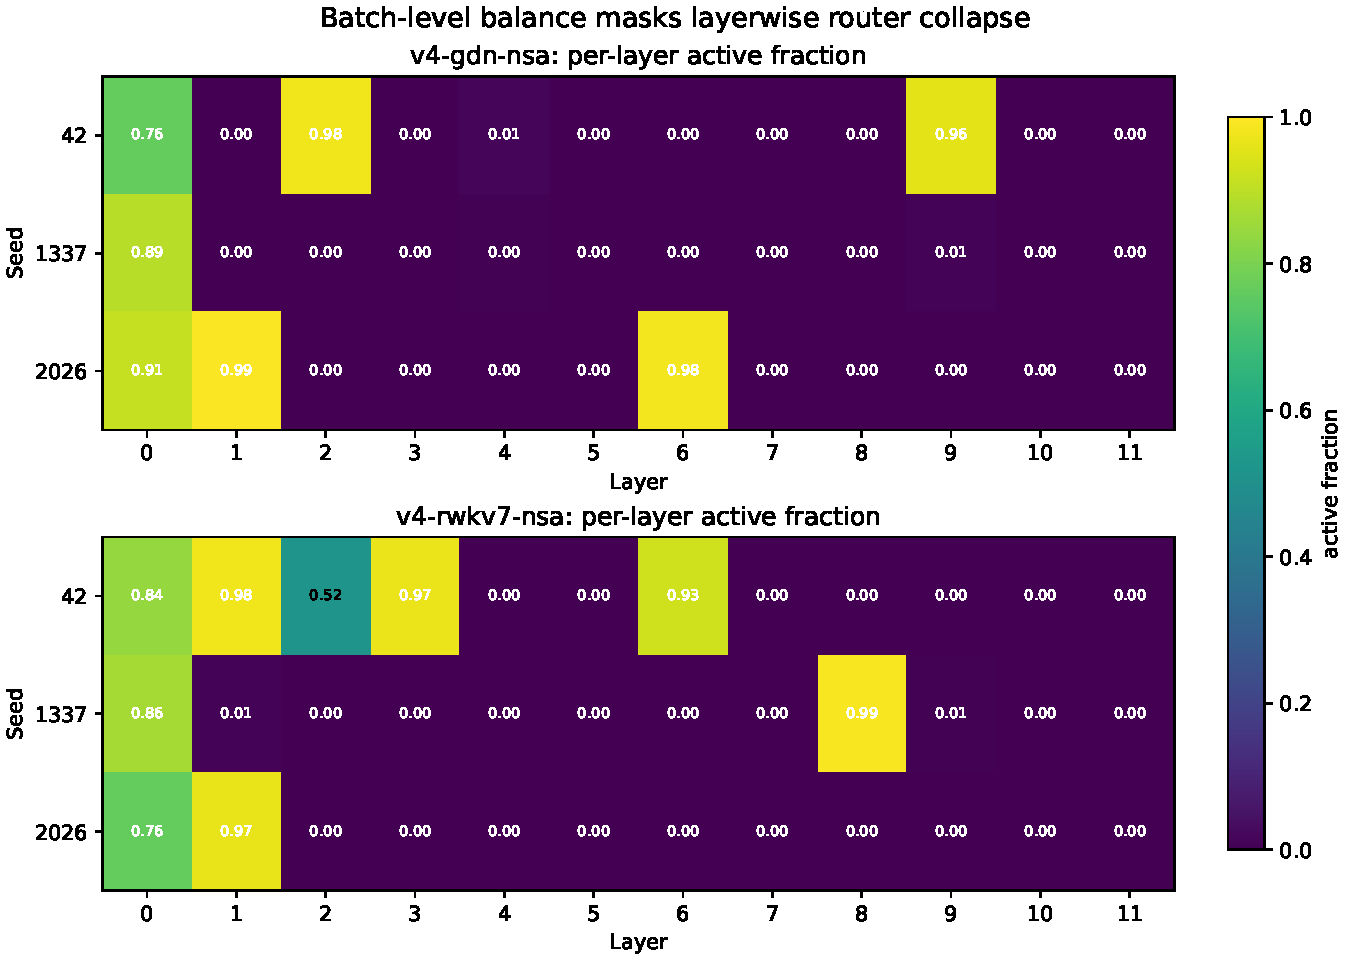
\includegraphics[width=0.66\textwidth]{figures/router_active_fraction_heatmap.pdf}
\caption{Per-layer router activity on the trained block-fusion checkpoint.
Batch-averaged statistics look on-target ($0.226$ vs $0.25$); per layer,
the router is all-or-nothing. Six layers never route, two more almost
never do; two route nearly everything.}
\label{fig:collapse}
\end{figure}

\section{350M: the advantage decays and the gate null repeats}
\label{sec:exp-350m}

Scale could rescue either story: maybe head fusion's edge grows, maybe
the gate finds signal once the model is big enough to expose it. Neither
happens.

\paragraph{Evaluation protocol.} Each 350M run reports the fresh
validation pass stored in its terminal checkpoint (32 freshly sampled
windows, about 262k tokens). In-loop periodic evaluations in the training
CSVs differ from this number by up to $\pm 2$ perplexity (different
random windows; for kill-clock-terminated runs, an earlier step). We use
the terminal-checkpoint number uniformly. A wall-clock kill-switch ended
some runs between steps 14{,}626 and 15{,}000, which is at least
$97.5\%$ of the cosine schedule, with the learning rate within $5\%$ of
its floor. Evaluation sampling noise of this size, comparable to the
cross-seed spread, is itself a finding: sub-2\% perplexity claims at this
scale, made from single seeds and single validation windows, should not
be trusted, including ours.

\begin{table}[t]
\centering
\begin{tabular}{lrr}
\toprule
Variant (350M) & PPL by seed (42/1337/2026) & mean $\pm$ std \\
\midrule
\texttt{hymba-with-nsa} (348.8M) & $87.38\;/\;86.99\;/\;81.60$ & $85.32 \pm 2.64$ \\
dense, $\mu$P (368.8M) & $84.23\;/\;80.18\;/\;86.82$ & $83.75 \pm 2.73$ \\
\midrule
\texttt{hymba-with-nsa-gated} & $78.25\;/\;89.06\;/\;79.75$ & $82.35 \pm 4.78$ \\
\texttt{hymba-with-nsa-randgate} & $82.93\;/\;85.73\;/\;82.73$ & $83.79 \pm 1.37$ \\
\bottomrule
\end{tabular}
\caption{350M results, 983M training tokens each. Top: the bare
architecture against dense. Bottom: learned against random gate. Neither
contrast is significant (Welch $t \approx 0.72$ and $-0.41$).}
\label{tab:350m}
\end{table}

\paragraph{Head fusion ties dense.} Table~\ref{tab:350m}, top:
$85.32 \pm 2.64$ vs $83.75 \pm 2.73$, a $+1.9\%$ nominal deficit with
fully overlapping intervals ($p \approx 0.5$), against a dense baseline
that carries 20M more parameters (configuration details in
Appendix~\ref{app:dense}). The $-3.4\%$ advantage from 140M is
gone (Fig.~\ref{fig:scaling}). We report this plainly because the
opposite claim, that a hybrid matches dense at one small scale and will
therefore hold at the next one, is common and, here, would have been
wrong. Zero-shot HellaSwag agrees: $0.275$ (hybrid) vs $0.285$ (dense)
on 1000 items against a $0.25$ random floor, both at the small-model
floor, separating nothing.

\begin{figure}[t]\centering
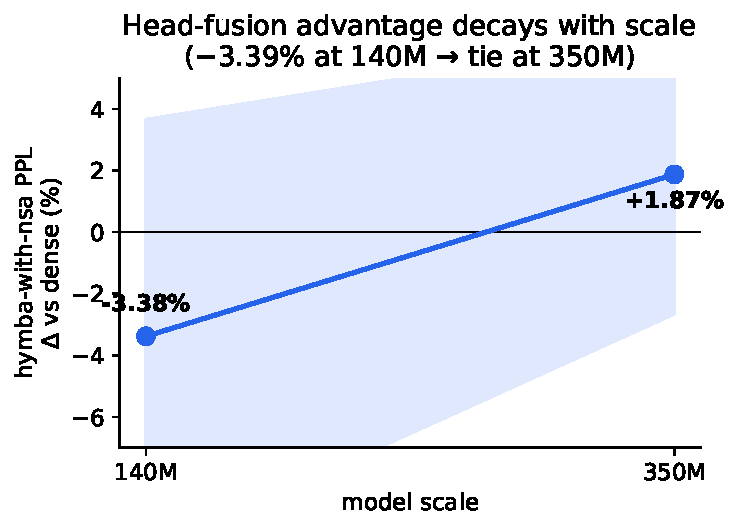
\includegraphics[width=0.6\textwidth]{figures/fig_scaling_advantage.pdf}
\caption{Head fusion's perplexity advantage over dense decays from
$-3.4\%$ at 140M to a statistical tie at 350M (3 seeds, Welch test).}
\label{fig:scaling}
\end{figure}

\paragraph{The gate null repeats, with a cautionary tale.}
Table~\ref{tab:350m}, bottom. The first 350M gated run we trained (seed
42) reached $78.25$, beating every base and dense seed by a wide margin,
and for a few days the working hypothesis was that the gate pays off at
scale. Then the remaining seeds came in: $89.06$ at seed 1337, the worst
of all six runs in the comparison. The learned gate's cross-seed spread
($\pm 4.78$) is $3.5\times$ the random gate's ($\pm 1.37$); the means are
statistically indistinguishable. The learned gate ties the random gate
at 350M, exactly as at 140M (Fig.~\ref{fig:gatenull}). We keep this
chronology in the paper because it is the cleanest illustration we have
of why the protocol demands seeds before claims.

\begin{figure}[t]\centering
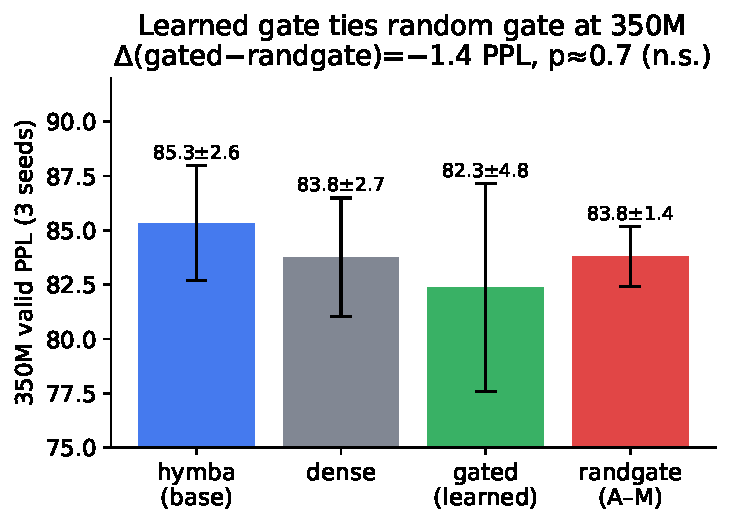
\includegraphics[width=0.6\textwidth]{figures/fig_gate_null_350m.pdf}
\caption{Learned vs random gate at 350M, 3 seeds each. The means tie; the
learned gate is the higher-variance way to get nothing.}
\label{fig:gatenull}
\end{figure}

So far this is two clean nulls and one retirement. The natural objection
is that some better gate, some better training scheme, would find the
signal. The rest of the paper measures whether any signal exists to find.

\section{The gate as a channel: an advantage bound}
\label{sec:theory}

Fix a layer and define, for each token $t$, the oracle routing label
\[
  s_t \;=\; \mathbf{1}\big[\,\LL_t(\text{attention stream ablated}) -
  \LL_t(\text{full model}) > 0\,\big],
\]
that is, ``the contextual stream lowers the next-token loss at $t$.'' The
label is a counterfactual on the stream's output and does not depend on
the gate's parameters. It is a marginal quantity: ablating one layer's
stream lets the trained downstream layers compensate, so $s_t$ measures
the stream's utility in the deployed network rather than in isolation,
which is the quantity a deployed gate actually faces. \S\ref{sec:limits}
discusses this choice. Write $p = \Pr[s_t{=}1]$ and $H(s)$ for its binary
entropy. A gate $g_t$, of any form, defines a channel $s \to g$, with
mutual information $I(g;s)$. Two mild assumptions. First, the ideal per-token benefit of routing
correctly is bounded by $\sigma_C^2/(2\LL)$, a second-order estimate: the
loss is locally quadratic in the stream's additive contribution, whose
mean squared norm is $\sigma_C^2$, normalised by the loss scale $\LL$.
This enters only as a prefactor and none of our conclusions depend on its
tightness. Second, routing the stream in on $s_t{=}0$ tokens is
non-beneficial in expectation.

\begin{proposition}[Gate-channel advantage bound]
\label{prop:channel}
With entropies in nats, any routing decision derived from $g_t$ has
advantage over chance capped by
\[
  \bigl(1 - 2P_{\mathrm{err}}\bigr)_+ \;\le\;
  \sqrt{2\bigl(I(g;s) + \log 2 - H(s)\bigr)} \;=:\; A(I),
\]
and its perplexity benefit over the always-on baseline is capped by
$\frac{\sigma_C^2}{2\LL}\, A(I)$. In particular, realising the full ideal
benefit ($A \geq 1$) requires
\[
  I(g;s) \;\geq\; \tfrac12 + H(s) - \log 2 \quad\text{nats},
\]
which is $\approx 0.72$ bits for a near-balanced label.
\end{proposition}

\begin{proof}
The chain $s \to g \to \hat{s}$ through any decision rule is Markov, so
Fano's inequality for a binary variable gives
$H(s \mid g) \le H_b(P_{\mathrm{err}})$ with
$H(s \mid g) = H(s) - I(g;s)$. Pinsker's inequality applied to
$\mathrm{Bern}(q)$ against $\mathrm{Bern}(\tfrac12)$ gives
$\log 2 - H_b(q) = D(\mathrm{Bern}(q)\,\Vert\,\mathrm{Bern}(\tfrac12))
\ge 2(q - \tfrac12)^2$, that is,
$H_b(q) \le \log 2 - 2(q-\tfrac12)^2$. Chaining the two,
$H(s) - I \le \log 2 - 2(P_{\mathrm{err}} - \tfrac12)^2$, which
rearranges to the advantage cap; the radicand is non-negative because
$H_b \le \log 2$ always. The loss reduction from routing is at most the
ideal selection benefit times the decision's advantage over chance, and
the ideal benefit is bounded by $\sigma_C^2/(2\LL)$ under the assumptions
above. Setting $A(I) \ge 1$ gives the threshold. A remark on a tempting
shortcut: the chord bound $H_b(q) \le 2q \log 2$, which would give a
sharper-looking linear threshold, is false on $(0, \tfrac12)$, since
$H_b$ is concave and lies above its chords. Pinsker provides the valid
direction.
\end{proof}

\begin{corollary}[The Aquino-Michaels null as a limit]
\label{cor:am}
A random gate has $I(g;s) = 0$, so its cap is
$\frac{\sigma_C^2}{2\LL}\sqrt{2(\log 2 - H(s))}$. For a balanced label
($H(s) = \log 2$) this is exactly zero: an uninformative gate provably
cannot beat always-on. For our measured label ($p = 0.445$,
$\log 2 - H(s) \approx 0.006$ nats) the $I{=}0$ cap is $A \approx 0.11$,
small but not zero; the corollary degrades gracefully. The modal collapse
of \S\ref{sec:h1} is the same corner reached differently: per-layer
$p_\ell \in \{0,1\}$ makes $H(s)$ per layer zero and leaves nothing to
discriminate.
\end{corollary}

The bound's value is that both sides are measurable. $H(s)$ and $I(g;s)$
come from counterfactual ablations and the gate's own values; no
curvature constants, no convexity assumptions on a trained network. (An
earlier curvature-based lower bound, retained in
Appendix~\ref{app:lambda} as corroboration, needed a Hessian-direction
constant $\lambda$ that is genuinely awkward to measure; the channel form
needs nothing of the sort.) The bound is also falsifiable in the strong
sense: if someone exhibits a gate with $I(g;s) \approx 0.7$ bits that
still fails, the assumptions are wrong; if every gate sits at $0.005$
bits, the observed nulls are forced.

\paragraph{The bound in plain terms.} A gate is a guesser. At every token
it guesses whether attention will earn its keep, and it can only guess
from what it sees. If the thing it is guessing is essentially a fair coin
given everything visible at that token, then no gate, however trained,
can beat the strategy of not guessing at all. Mutual information is
simply the honest score of how much better than a coin the gate could
possibly be, and the proposition converts that score into a hard cap on
perplexity benefit. The rest of the paper measures the score.

\section{Measuring the channel: two decades short, with a ceiling}
\label{sec:ceiling}

\subsection{What trained gates carry}
\label{sec:mi}

We estimate $I(g;s)$ with a Miller-Madow bias-corrected plug-in estimator
\citep{miller1955}, self-tested
before use (independent variables give $0.0006$ bits, a deterministic
relation gives $0.9999$). The label $s$ uses per-layer NSA ablation on
held-out text.

\begin{table}[t]
\centering
\begin{tabular}{lcc}
\toprule
$I(g;s)$ in bits & learned gate & random gate \\
\midrule
140M (3 seeds) & $0.0059 \pm 0.0004$ & $0.0029 \pm 0.0006$ \\
350M & $0.0040$ & $0.0021$ \\
\midrule
full-benefit threshold & \multicolumn{2}{c}{$\approx 0.72$ bits} \\
\bottomrule
\end{tabular}
\caption{Gate-channel mutual information against the threshold of
Proposition~\ref{prop:channel}. The parameter-free PC gate measures
$0.0072$ bits at 140M (single seed), the highest of the three gate
types.}
\label{tab:mi}
\end{table}

Three observations from Table~\ref{tab:mi} and Fig.~\ref{fig:mi}.
First, the learned gate does learn something: twice the random
gate's information, with non-overlapping 3-seed intervals, at both
scales. Second, a circularity check: since $s$ is measured on the same
model that hosts the gate, we recomputed $I$ with the label taken from an
independently trained gate-free model that the gate never influenced.
The separation survives unchanged ($0.0055$ vs $0.0028$ bits), so the
ordering is not a self-measurement artefact. Third, none of it matters
for perplexity: $0.006$ bits against a $0.72$-bit threshold is two
orders of magnitude short. Substituted into the advantage cap, the
learned gate can realise at most $14\%$ of the ideal routing benefit,
the random gate $13\%$, the PC gate $15\%$. The $2\times$ information
separation collapses to two points of advantage because the
near-balance slack $\log 2 - H(s)$ dominates both. The bound therefore
predicts: no visible perplexity difference between any of these gates,
at either scale. That is what Tables~\ref{tab:140m} and \ref{tab:350m}
show.

\begin{figure}[t]\centering
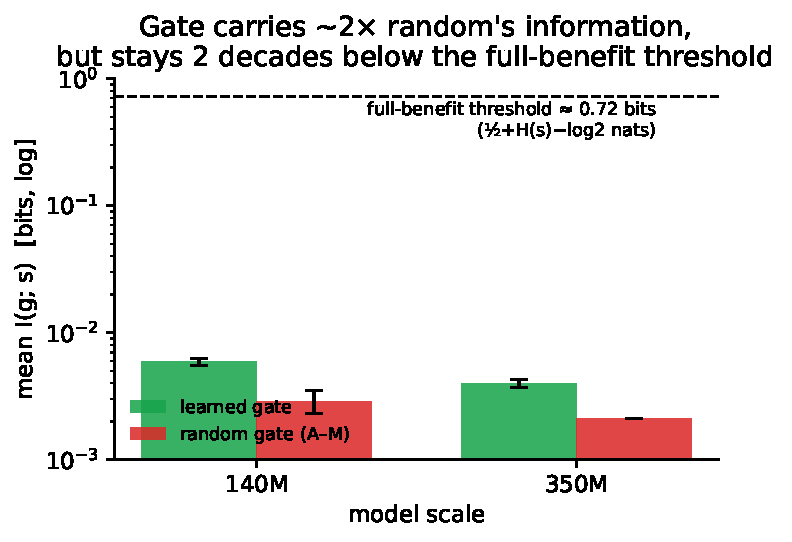
\includegraphics[width=0.6\textwidth]{figures/fig_mi_threshold.pdf}
\caption{Measured gate information (log scale) against the full-benefit
threshold. Learned beats random by $2\times$ at both scales and both
are two decades below threshold, so the bound predicts the observed
perplexity null.}
\label{fig:mi}
\end{figure}

\subsection{What any gate could carry: the ceiling}
\label{sec:ceiling-probe}

The trained gates might just be badly trained. To close that escape, we
train probes \emph{directly on the oracle label}, with a 70/30 split and
held-out evaluation, giving them strictly more than any gate in this
class gets: (a) a linear probe on the residual $h_t$, the gate's actual
input; (b) an MLP on the concatenation of $h_t$, both streams' per-head
output norms, and their difference. The held-out $I(\text{probe}; s)$ is
the ceiling for any gate computable from token-local features.

\begin{center}
\begin{tabular}{llcc}
\toprule
probe & features & held-out $I$ & val.\ accuracy \\
\midrule
linear & $h_t$ & $0.0315$ bits & $0.54$ to $0.68$ \\
MLP (64 hidden) & $[\,h_t, \norm{C}, \norm{R}, \norm{C}{-}\norm{R}\,]$ & $0.0341$ bits & $0.55$ to $0.65$ \\
\bottomrule
\end{tabular}
\end{center}

The ceiling is $0.034$ bits at the default probe capacity, and it is
robust to the two objections a careful reader should raise. Probe
capacity: quadrupling the MLP width (64 to 256 hidden units) moves the
ceiling from $0.034$ to $0.037$ bits, an $8\%$ change, so the probe is
not underfit in any way that matters against a $0.72$-bit threshold.
Split variance: across four independent train/validation splits the
ceiling spans $0.030$ to $0.034$ bits. Taking the most favourable value
for routing, $0.037$ bits, the ceiling sits about $20\times$ below the
threshold, an advantage cap of $A \le 0.25$ for \emph{any} token-local
gate, linear or not, supervised or not (Fig.~\ref{fig:ceiling}). The
nonlinear probe with access to both streams' outputs does scarcely
better than a linear readout of the residual; held-out accuracy barely
clears the base rate. The trained gates sit a further $6$ to $8\times$
below their own ceiling, so better gate training could close that last
gap and still change nothing.

The conclusion is structural. The event ``attention helps at this token''
is nearly information-free given everything a per-token gate can see,
including the streams' own outputs. At the token level the two streams
are, on this corpus, almost interchangeable. Absorption is not the
optimiser failing to find the good gate; there is no good gate.

\begin{figure}[t]\centering
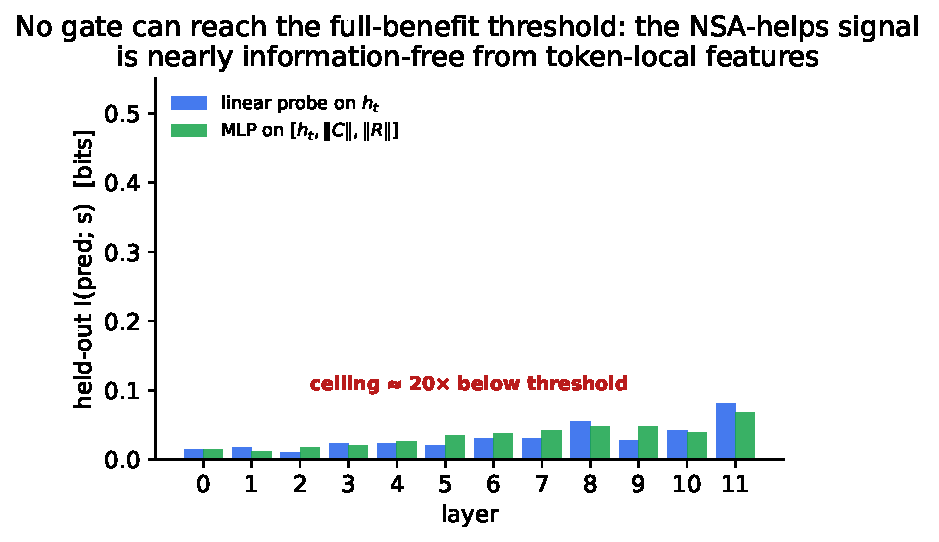
\includegraphics[width=0.62\textwidth]{figures/fig_gate_ceiling.pdf}
\caption{Held-out information ceiling for optimal probes trained directly
on the oracle label, per layer, against the full-benefit threshold. Even
the nonlinear probe on both streams' outputs sits about $20\times$ below.}
\label{fig:ceiling}
\end{figure}

\subsection{The optimal policy is always-on}
\label{sec:always-on}

One question remains: maybe the routing signal lives at a coarser
granularity. We ablated the entire attention stream per sequence on 256
held-out sequences. It hurts on all 256, by $405 \pm 111$ summed nats
(range 107 to 830), never once helping. Decomposing the per-token benefit
variance: $1.1\%$ between sequences, $98.9\%$ within. So sequence- or
segment-level routing has even less to work with than token-level
routing, and the within-sequence part is exactly the $0.03$-bit signal
the ceiling already measured.

Putting the pieces together: the contextual stream helps almost
everywhere, and the only deviations from ``everywhere'' are nearly
unpredictable from anything a gate can see. Within the class of policies
that act on token-local features, nothing can improve on the constant
policy by more than the ceiling's $0.03$-bit residual allows, so the optimal
member of that class is, to within measurement precision, always on. Always-on is the gate-less baseline. Every gate in this
paper could only tie it or lose to it, and that is what every gate did.
The gate fails not because routing is hard but because, on this data,
routing is trivial.

\section{The constructive programme: a routability phase diagram}
\label{sec:programme}

A measured impossibility earns its keep by saying exactly what would make
the impossible possible. The bound identifies two levers and only two:
raise $H(s)$ structure that a gate can see (the data lever), or make the
streams non-redundant so that $s$ becomes decodable (the architecture
lever). We committed both to a falsifiable experimental programme,
released as a runnable queue (\texttt{run\_v6\_queue.py}, two GPU-days on
the same hardware), with the predictions below frozen in the queue header
before any run started. \S\ref{sec:programme-results} reports the
outcome.

\paragraph{The data lever.} Construct mixture corpora that interleave
wikitext prose with synthetic key-value recall segments at a controlled
token fraction $\pi \in \{0, 0.1, 0.25, 0.5\}$. Inside a recall segment,
answering a query requires exact associative recall across roughly a
hundred tokens: attention is decisive there by construction, while a
fixed-state recurrence saturates; on prose the streams are substitutable,
as this paper measured. The corpus dial $\pi$ therefore directly
controls how much routable structure exists.

\paragraph{The architecture lever.} A stream-decorrelation regulariser:
the squared cross-correlation between the attention heads' and SSM heads'
token-level output features, added to the loss with a small coefficient
(a Barlow-Twins-style cross term applied across streams rather than
augmented views). If per-token routing fails because the streams are
redundant, then forcing decorrelation should make ``which stream helps''
decodable, raising the measured ceiling at fixed data.

\paragraph{Pre-registered predictions.}
\begin{itemize}
\item \textbf{P1.} The optimal-probe ceiling $I_{\max}(\pi)$ rises
      monotonically with $\pi$, measured before the perplexity
      comparisons complete.
\item \textbf{P2.} Learned gate separates from the frozen-random gate
      (3-seed intervals) only at the $\pi$ where $I_{\max}$ approaches
      the threshold of Proposition~\ref{prop:channel}; at $\pi = 0$ the
      null of this paper must reproduce.
\item \textbf{P3.} Any gate benefit concentrates at recall-answer
      positions; background-prose loss shows no gate effect at any
      $\pi$.
\item \textbf{P4.} Decorrelation raises $I_{\max}$ at fixed $\pi$. If it
      raises the ceiling but perplexity does not follow where P2 says it
      should, the redundancy explanation is wrong and the bound's
      premise fails.
\end{itemize}

Falsification is symmetric and cheap. If $I_{\max}$ stays flat in $\pi$,
the ``data is the lever'' claim dies; if the gate separates where the
ceiling says it cannot, the bound dies. Either outcome closes the loop
the null results opened, which is what makes the programme worth
running: the theory has committed to numbers in advance.

\subsection{Programme results: the ceiling moves, the bound holds}
\label{sec:programme-results}

The queue completed after the predictions above were frozen (63 training
runs, 3 seeds each, the 140M recipe on 60M-token mixture streams; these
perplexities are internally comparable across variants but not to
Table~\ref{tab:140m}, which used the full corpus).

\begin{table}[t]
\centering
\begin{tabular}{lrrrr}
\toprule
 & $\pi{=}0$ & $\pi{=}0.10$ & $\pi{=}0.25$ & $\pi{=}0.50$ \\
\midrule
ceiling $I_{\max}(\pi)$ [bits] & $0.018$ & $0.058$ & $0.108$ & $0.139$ \\
\midrule
gate-less PPL      & $111.9 \pm 3.6$ & $109.6 \pm 1.6$ & $103.2 \pm 3.1$ & $88.7 \pm 2.9$ \\
PC gate            & $114.7 \pm 4.7$ & $110.6 \pm 1.0$ & $101.1 \pm 1.8$ & $\mathbf{87.3 \pm 1.0}$ \\
learned gate       & $116.0 \pm 2.5$ & $110.3 \pm 2.3$ & $104.1 \pm 3.1$ & $92.6 \pm 2.5$ \\
random gate        & $115.6 \pm 3.5$ & $111.8 \pm 1.7$ & $105.0 \pm 1.0$ & $90.7 \pm 4.4$ \\
\midrule
gate MI: learned   & $0.003$ & $0.004$ & $0.041$ & $0.033$ \\
gate MI: random    & $0.003$ & $0.003$ & $0.015$ & $0.022$ \\
\bottomrule
\end{tabular}
\caption{Routability phase diagram, executed. Top: the optimal-probe
ceiling rises $7.9\times$ with the recall fraction $\pi$, yet stays
$5\times$ below the $0.72$-bit threshold even at $\pi = 0.5$. Middle:
validation perplexity (3 seeds). Bottom: non-circular gate mutual
information in bits.}
\label{tab:v6}
\end{table}

\begin{figure}[t]\centering
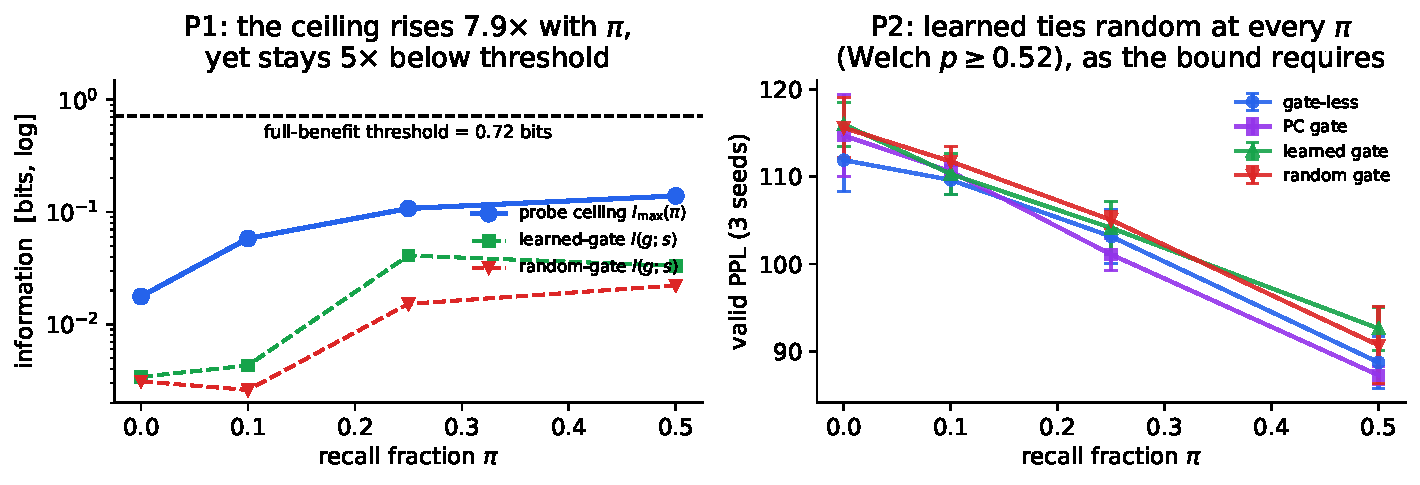
\includegraphics[width=\textwidth]{figures/fig_v6_phase.pdf}
\caption{The executed phase diagram. Left: information against the
recall fraction $\pi$ (log scale). The probe ceiling and both gates'
mutual information rise with $\pi$; none approaches the threshold.
Right: perplexity by variant. The learned and random gates stay
statistically tied at every $\pi$, and the parameter-free PC gate
tracks or beats the gate-less baseline.}
\label{fig:v6}
\end{figure}

\textbf{P1 confirmed.} The ceiling rises monotonically,
$0.018 \to 0.058 \to 0.108 \to 0.139$ bits (Table~\ref{tab:v6},
Fig.~\ref{fig:v6} left): the routing target's information content is a
controllable, monotone function of data composition. What the main paper
established by measurement, the diagram establishes by intervention. The
trained gates follow: learned-gate MI grows $12\times$ (to $0.041$ bits
at $\pi = 0.25$), holding a $2$--$3\times$ margin over the random
control.

\textbf{P2 confirmed on its testable branch.} Even at $\pi = 0.5$ the
ceiling sits $5\times$ short of the threshold, so the bound predicts
that the learned gate still cannot separate from random. It does not:
Welch $p \in [0.52, 0.90]$ at every $\pi$, and the $\pi = 0$ null of the
main paper reproduces ($p = 0.90$). The diagram never reached the regime
where P2's positive branch could fire. The obvious follow-up is to push
$\pi$ or the segment design until $I_{\max}$ crosses $0.72$ bits, where
the bound finally permits, and P2 then demands, a gate win.

\textbf{P3: no gate benefit anywhere, and a caveat.} Answer-position
loss is statistically identical across all six variants at every $\pi$.
The caveat: at this training budget (98M tokens) no variant actually
solved the recall task (answer-position CE $21$--$27$ nats against a
$10.8$-nat uniform baseline), so the diagram explored the regime where
the routing signal exists but the capability it routes toward is still
unlearned. The regime where recall is solved and routing could pay is
open, and requires longer training, not a different gate.

\textbf{P4 falsified: the architecture lever, as implemented, fails.}
Stream decorrelation does not raise the ceiling ($0.094$ vs $0.108$ bits
at $\pi = 0.25$) and leaves perplexity unchanged ($103.1 \pm 2.3$ vs
$103.2 \pm 3.1$). Output-feature decorrelation is evidently not the same
thing as functional specialisation; the redundancy that kills routing is
not expressible as a cross-correlation penalty. A pre-registered
prediction failed, and we report it as such.

\textbf{An unregistered but consistent finding.} Pooled across the
diagram (paired over $\pi \times$ seed, $n = 12$), the parameter-free PC
gate beats the learned gate by $2.35$ perplexity ($p = 0.041$) while
tying the gate-less baseline ($p = 0.95$). The ordering gate-less
$\approx$ PC $>$ learned $\approx$ random, already visible at 140M in
Table~\ref{tab:140m}, persists across the whole phase diagram: a gate
with no trainable parameters costs nothing, while a trainable gate pays
an interference tax that grows with $\pi$ ($+3.9$ perplexity over
gate-less at $\pi = 0.5$). If a design must gate, it should gate without
parameters. We flag this as post-hoc; it awaits its own pre-registered
test.

\section{Discussion}
\label{sec:discussion}

\paragraph{One lens for three results.} The router collapse
(\S\ref{sec:h1}), the 140M gate null, and the 350M gate null look like
three separate failures. The channel view unifies them: all three are
gates asked to discriminate an event that carries about $0.03$ bits of
decodable signal. The block-fusion router additionally destroys its own
label by collapsing $p_\ell$ to $\{0,1\}$, which is why block fusion does
not merely tie the baseline but loses outright: it pays the full
apparatus cost (parameters, FLOPs, optimisation interference, dead
layers) for a discrimination task that was nearly empty to begin with.

\paragraph{What would make routing work.} The bound points away from
gate engineering and toward the data. The label $s_t$ is nearly constant
because uniform web prose exercises both streams on almost every token.
Corpora where the streams genuinely specialise, for instance long-range
retrieval interleaved with local prose, key-value recall tasks, or code
with distant references, are exactly where $H(s)$ grows and $s$ becomes
predictable from context. The honest statement of scope: on wikitext-style
data at sub-2B scale, per-token attention-vs-SSM routing is dead on
arrival, and a probe of the oracle label would have told us so before
training a single router. We offer that probe as a cheap pre-flight check
for any adaptive-compute proposal: measure the ceiling first.
\S\ref{sec:programme-results} backs this by intervention: raising the
corpus recall density raises the ceiling on cue, and every null stays
where the sub-threshold ceiling forces it.

\paragraph{Relation to the concurrent routing literature.} Our reading
of the 2026 cluster (\S\ref{sec:related}) is that the field is
independently converging on routing scepticism from several directions:
topology equifinality, counterfactual uninformativeness, low-rank routing
subspaces. The gate-channel bound supplies what those reports lack, a
quantitative necessary condition, and the ceiling probe supplies the
measurement that decides it. The combination upgrades ``routers do not
seem to specialise'' to ``no token-local router can, here, by this
margin.''

\paragraph{Limitations.}
\label{sec:limits}
Everything was trained on one consumer GPU. That caps the study at 350M
parameters and about $10^9$ tokens per run, on multi-epoch wikitext-103;
a fresh-corpus run at the 5B-token Chinchilla bracket remains open, and
our scaling statement (the 140M advantage decays by 350M) is two points
on a curve, not a law. The ceiling measurement covers one architecture
class and two corpus families (uniform prose and the synthetic mixtures
of \S\ref{sec:programme-results}); natural retrieval-heavy corpora
remain untested. Zero-shot HellaSwag is at the
small-model floor for every variant, separating nothing at this scale.
A needle-in-a-haystack probe returned zero for all models; we attribute
this to the probe demanding verbatim multi-token generation from a small
base LM rather than to retrieval capacity, and rely on multi-query
associative recall (MQAR; \citealp{zoology}) for recall signal instead
(Appendix~\ref{app:synthetics}). Evaluation
sampling noise at 350M is about $\pm 2$ perplexity, the same order as
cross-seed spread; both bound the resolution of any claim in
Table~\ref{tab:350m}. Two caveats specific to the phase diagram of
\S\ref{sec:programme-results}: mixture-corpus perplexities are not
comparable to the main 140M table (different stream construction and
token budget), and part of the perplexity drop with $\pi$ reflects the
predictable padding inside recall segments rather than solved recall;
the answer positions themselves were never learned at this budget, so
the high-$\pi$, recall-solved regime remains unexplored.
The oracle label is defined by single-layer ablation inside the trained
network, so it measures marginal utility given downstream compensation;
a label defined against independently trained reduced models could
differ, although the whole-stream sequence ablation of
\S\ref{sec:always-on}, which removes all layers' attention at once and
still hurts on every sequence, bounds how much compensation can be doing.
Finally, the advantage cap's prefactor $\sigma_C^2/(2\LL)$ is an
upper-bound constant, not a tight prediction of effect size; the bound's
force is in the threshold and the measured ceiling, not in the
prefactor.

\section{Conclusion}

We set out to build a better router for hybrid attention-SSM language
models and ended up measuring why no such router can exist on this data.
Block fusion with a learned router loses $19.5\%$ perplexity to plain
head fusion and its router modally collapses. The learned per-token gate
ties a frozen random gate at 140M and at 350M. The gate-channel bound
says a gate needs about $0.72$ bits of information about where attention
helps; trained gates carry $0.005$, and an optimal probe trained on the
oracle label itself tops out near $0.035$, because ablating attention
hurts on every single sequence and almost all benefit variance is
unpredictable within-sequence noise. The optimal policy is always-on,
the gate-less baseline wins by construction, and the right response to
routing absorption at this scale is not a cleverer gate but no gate,
plus data on which the question is worth asking.

We release the probe, the estimators, and all per-seed numbers, so the
next routing proposal can check in an afternoon, before training,
whether its target carries enough information to route on. We also
release the routability programme of \S\ref{sec:programme}, whose
pre-registered predictions the theory survived: the ceiling moved
$7.9\times$ when the data demanded it, the nulls landed where the bound
put them, and the one prediction that failed, decorrelation as a
specialisation mechanism, failed in the open.

\paragraph{Reproducibility.} All training runs, probes, and estimators
are scripted in the accompanying repository; Appendix~\ref{app:repro}
maps every number in this paper to its source log or checkpoint. The
hardware budget for the full study, 134 training runs plus diagnostics,
was one RTX 5090 for roughly three GPU-weeks.

\appendix

\section{Per-layer router diagnostic (block fusion, 154M, seed 42)}
\label{app:router}

Gate statistics over 8 validation batches of $4 \times 1024$ tokens,
\texttt{v4-gdn-nsa} at the best learning rate. ``Active'' means gate
$> 0$.

\begin{center}
\begin{tabular}{rrrrl}
\toprule
Layer & active frac. & gate mean & gate std & state \\
\midrule
0 & 0.764 & 0.030 & 0.029 & functioning \\
1 & 0.000 & 0.000 & 0.000 & dead \\
2 & 0.980 & 3.423 & 1.029 & saturated \\
3 & 0.000 & 0.000 & 0.000 & dead \\
4 & 0.012 & 0.421 & 3.690 & rare spikes \\
5 & 0.000 & 0.000 & 0.000 & dead \\
6 & 0.0002 & 0.0001 & 0.006 & nearly dead \\
7 & 0.000 & 0.000 & 0.000 & dead \\
8 & 0.000 & 0.000 & 0.000 & dead \\
9 & 0.957 & 47.22 & 316.2 & saturated, unstable \\
10 & 0.00003 & 0.00001 & 0.0006 & nearly dead \\
11 & 0.000 & 0.000 & 0.000 & dead \\
\bottomrule
\end{tabular}
\end{center}

Mean active fraction $0.226$ (target $0.25$): the balancer satisfies its
objective by averaging extremes. The RWKV-7 block-fusion variant shows
the same pattern (4 dead layers, 5 nearly dead, mean $0.353$).

\section{Curvature corroboration: the $\lambda$ bound}
\label{app:lambda}

Before the channel formulation we proved a curvature-based lower bound,
$\rho - 1 \geq \lambda \sigma_C^2 p(1-p)\gamma^2 / (2\LL)$, where $\rho$
is the random-to-learned loss ratio, $\gamma$ the gate saturation margin
(whose growth under gradient descent follows the implicit-bias analysis
of \citealp{soudry2018}),
and $\lambda$ the loss curvature along the gate-action direction. Its
weakness is $\lambda$: a naive finite difference over the
high-dimensional gate-parameter space collapses to zero under BF16
rounding (each coordinate perturbation falls below the loss's unit in
the last place), and the global smallest Hessian eigenvalue of a trained
network is typically non-positive, which makes a strong-convexity
reading fragile. Measuring instead the curvature along a single scalar
gate-gain axis in FP32 (a 5-point stencil, self-tested on $f(x)=x^2$)
gives $\lambda = 0.186$ on the 140M learned-gate checkpoint, with
$\sigma_C = 9.77$, $p = 0.445$, $\gamma = 0.550$, $\LL = 5.00$, hence
$\rho_{\mathrm{LB}} - 1 \approx 0.13$, non-vacuous and correctly signed
against the measured $+1.7\%$ learned-vs-random gap. We report this as
corroboration only; every headline claim uses the channel bound, which
needs no curvature constant.

\section{Dense 350M baseline details}
\label{app:dense}

Dense, $\mu$P-style initialisation, 24 layers, width 1024, 16 heads, 4 KV
heads, 368.79M parameters, same recipe and token budget as the hybrid:
seeds $\{42,1337,2026\}$ give perplexity $84.23 / 80.18 / 86.82$, mean
$83.75 \pm 2.73$. Throughput $\approx 43{,}000$ tok/s at BF16 on the RTX
5090, peak VRAM 13.9 GB (the hybrid: $\approx 27{,}000$ tok/s, 20.6 GB).

% Comprehensive appendix tables - sourced verbatim from results/:
%   phase2_param_breakdown_2026-05-12.md, phase2_flops_140m_2026-05-12.md,
%   phase2_synthetics_table_2026-05-12.md. \input near the end of the paper.

\section{Whole-model parameter accounting (140M config)}
\label{app:params}
12 layers, $d{=}768$, $H{=}12$, $H_{kv}{=}4$, vocab 50{,}257 (GPT-2 BPE).

\begin{center}
\begin{tabular}{lrrrr}
\toprule
Variant & Embed & 12 blocks & LM head & Total \\
\midrule
\texttt{dense} & 38.60M & 75.52M & 38.60M & \textbf{152.71M} \\
\texttt{hymba} & 38.60M & 115.65M & tied & 154.25M \\
\texttt{hymba-with-nsa} & 38.60M & 115.73M & tied & 154.33M \\
\texttt{v4-gdn-nsa} & 38.60M & 116.11M & tied & 154.71M \\
\texttt{v4-rwkv7-nsa} & 38.60M & 130.31M & tied & 168.91M \\
\bottomrule
\end{tabular}
\end{center}

Per-block Q/K/V/O projection share: dense/hymba/hymba-with-nsa $\approx$
1.57--1.77M; \texttt{v4-*} block-fusion $\approx$ 2.56M (decoupled per-stream
Q/K/V). The $+19.47\%$ head-vs-block PPL gap is not explained by this $<1\%$
total-parameter difference (all variants are matched at $\approx154$M except
\texttt{v4-rwkv7-nsa}); it is structural, consistent with the router-collapse
diagnostic (\S\ref{sec:h1}).

\section{Forward-pass FLOPs at the 140M config}
\label{app:flops}
Counted with \texttt{torch.utils.flop\_counter} at $S{=}1024$, batch 1.
The $2P$ column is the Kaplan forward approximation ($2\times$ params).

\begin{center}
\begin{tabular}{lrrr}
\toprule
Variant & Params (M) & Fwd FLOPs/tok (M) & $\Delta$ vs $2P$ \\
\midrule
\texttt{dense} & 152.71 & 228.2 & $-25.3\%$ \\
\texttt{hymba} & 154.25 & 345.6 & $+12.0\%$ \\
\texttt{hymba-with-nsa} & 154.33 & 365.8 & $+18.5\%$ \\
\texttt{hymba-with-asa} & 154.27 & 355.1 & $+15.1\%$ \\
\texttt{hymba-with-nsa-select} & 154.33 & 368.5 & $+19.4\%$ \\
\texttt{v4-gdn-nsa} & 154.71 & 435.4 & $+40.7\%$ \\
\texttt{v4-rwkv7-nsa} & 168.91 & 389.5 & $+15.3\%$ \\
\bottomrule
\end{tabular}
\end{center}

NSA's compress + sliding-window branches add $O(S^2)$ compute over the $2P$
base; ASA (no compress) is cheaper; the PC gate is negligible. Block-fusion
(\texttt{v4-gdn-nsa}, $+40.7\%$) runs a separate full contextual stream and a
separate reflexive stream, the most expensive of all.

\section{Small-scale state-tracking battery}
\label{app:synthetics}
$\approx$1.7--2.8M params, 4 layers, $d{=}128$, 2000 steps. Reviewer-C
expressivity probe. ($\star$ = best per task.)

\begin{center}
\begin{tabular}{lrrr}
\toprule
Variant & MQAR acc & Dyck-2 PPL & Parity acc \\
\midrule
\texttt{dense} & 0.02\% & 2.737 & 50.86\% \\
\texttt{v4-gdn-nsa} & 0.72\% & 2.590 & 52.41\%$^\star$ \\
\texttt{v4-mamba3-nsa} & 0.71\% & 2.646 & 50.58\% \\
\texttt{v4-rwkv7-nsa} & 1.03\%$^\star$ & 2.565$^\star$ & 52.15\% \\
\texttt{hymba} & 0.12\% & 2.693 & 50.73\% \\
\texttt{hymba-with-nsa} & 0.37\% & 2.677 & 50.59\% \\
\texttt{hymba-with-nsa-gated} & 0.23\% & 2.635 & --- \\
\texttt{hymba-with-nsa-randgate} & 0.02\% & 2.656 & --- \\
\texttt{hymba-with-asa} & 0.06\% & 2.679 & 51.09\% \\
\bottomrule
\end{tabular}
\end{center}

The RWKV-7 generalised delta rule leads MQAR (state tracking) and Dyck-2;
parity sits at chance ($\sim$50\%) for every variant, consistent with the
TC$^0$ ceiling at this tiny scale. At 1.7M the gate apparatus burns capacity
without payback (the gated-vs-randgate gap is within noise), consistent with
the absorption analysis at 140M/350M.


\section{Reproduction map}
\label{app:repro}

Every number above traces to a logged artefact in the repository:
the 140M table to \texttt{results/phase2\_combined\_140m\_2026-05-12.md}
and the per-run CSVs under \texttt{checkpoints\_p2screen/},
\texttt{checkpoints\_p2b/}, \texttt{checkpoints\_p2c/} (PC gate), and
\texttt{archive/checkpoints/checkpoints\_p2d/} (select);
the 350M tables to the terminal checkpoints under
\texttt{checkpoints\_p4\_350m*/}, \texttt{checkpoints\_p4b\_dense*/},
\texttt{checkpoints\_p4\_gated\_s*/}, \texttt{checkpoints\_p4\_randgate\_s*/};
the router diagnostic to \texttt{diagnose\_v4\_router.py};
mutual information to \texttt{measure\_gate\_channel\_mi.py}
(self-tests included) and \texttt{results/theorem\_empirics\_2026-06-02.md};
the ceiling probes to \texttt{probe\_gate\_ceiling.py},
\texttt{probe\_gate\_ceiling2.py}, and
\texttt{results/gate\_ceiling\_finding\_2026-06.md};
the sequence ablation to \texttt{probe\_sequence\_routing.py};
FLOPs to \texttt{profile\_flops\_140m.py};
$\lambda$ to \texttt{measure\_theorem\_constants.py};
HellaSwag to \texttt{eval\_hellaswag.py};
the \S\ref{sec:programme} programme to \texttt{build\_mix\_corpus.py},
\texttt{run\_v6\_queue.py}, \texttt{eval\_mix\_split.py}, and
\texttt{aggregate\_v6.py} (predictions frozen in the queue header before
execution).
Training used PyTorch 2.10 (cu128), Triton 3.6, and
flash-linear-attention 0.5.0 on driver 580.95.

\begin{thebibliography}{99}

\bibitem[Aquino-Michaels(2026)]{absorption2026} Aquino-Michaels, K.
Routing Absorption in Gated Dual-Stream Language Models.
arXiv:2603.02227, 2026.

\bibitem{hymba} Dong, X., Fu, Y., Diao, S., et al. Hymba: A Hybrid-head
Architecture for Small Language Models. ICLR 2025. arXiv:2411.13676.

\bibitem{jamba} Lieber, O., Lenz, B., Bata, H., et al. Jamba: A Hybrid
Transformer-Mamba Language Model. arXiv:2403.19887, 2024.

\bibitem{mor} Bae, S., et al. Mixture-of-Recursions: Learning Dynamic
Recursive Depths. NeurIPS 2025. arXiv:2507.10524.

\bibitem{mamba2} Dao, T., Gu, A. Transformers are SSMs: Generalized
Models and Efficient Algorithms Through Structured State Space Duality.
ICML 2024. arXiv:2405.21060.

\bibitem{mamba3} Lahoti, A., et al. Mamba-3: Improved Sequence Modeling
using State Space Principles. ICLR 2026. arXiv:2603.15569.

\bibitem{rwkv7} Peng, B., et al. RWKV-7 ``Goose'' with Expressive
Dynamic State Evolution. arXiv:2503.14456, 2025.

\bibitem{gateddeltanet} Yang, S., Kautz, J., Hatamizadeh, A. Gated Delta
Networks: Improving Mamba2 with Delta Rule. ICLR 2025. arXiv:2412.06464.

\bibitem{nsa} Yuan, J., et al. Native Sparse Attention:
Hardware-Aligned and Natively Trainable Sparse Attention.
arXiv:2502.11089, 2025.

\bibitem{asa} Hu, Y., et al. Alternating Sparse Attention.
arXiv:2511.00819, 2025.

\bibitem{videonsa} VideoNSA: Native Sparse Attention Scales Video
Understanding. arXiv:2510.02295, 2025.

\bibitem{remoe} Wang, Z., Zhu, J., Chen, J. ReMoE: Fully Differentiable
Mixture-of-Experts with ReLU Routing. ICLR 2025. arXiv:2412.14711.

\bibitem{deepseekv3} DeepSeek-AI. DeepSeek-V3 Technical Report.
arXiv:2412.19437, 2024.

\bibitem{stmoe} Zoph, B., et al. ST-MoE: Designing Stable and
Transferable Sparse Expert Models. arXiv:2202.08906, 2022.

\bibitem{sdt} Wieser, M., Benfeghoul, A., Bou Ammar, H., et al.
Subjective Depth and Timescale Transformers: Learning Where and When to
Compute. arXiv:2511.21408, 2025.

\bibitem{cir} Tang, Z. Compression is Routing: Reconstruction Error as
an Intrinsic Signal for Modular Language Models. arXiv:2512.16963, 2025.

\bibitem{dmem} Song, Y., Xin, Q. D-MEM: Dopamine-Gated Agentic Memory
via Reward Prediction Error Routing. arXiv:2603.14597, 2026.

\bibitem{selfrouting} Mohamud, A., Wagner, D., Ravanelli, M.
Self-Routing: Parameter-Free Expert Routing from Hidden States.
arXiv:2604.00421, 2026.

\bibitem[Ternovtsii and Bilak(2026)]{equifinality} Ternovtsii, O.,
Bilak, R. Equifinality in Mixture of Experts: Routing Topology Does Not
Determine Language Modeling Quality. arXiv:2604.14419, 2026.

\bibitem{counterfactual2026} Counterfactual Routing Analysis: Routers
are Uninformative on Hard Tokens. arXiv:2605.07260, 2026.

\bibitem{mythspec2026} The Myth of Expert Specialization in
Mixture-of-Experts Models. arXiv:2604.09780, 2026.

\bibitem{routingparadox2026} The Routing Paradox: Expert Selection Lives
in a Low-Dimensional Subspace. arXiv:2603.20997, 2026.

\bibitem[Soudry et al.(2018)]{soudry2018} Soudry, D., Hoffer, E.,
Nacson, M.S., Gunasekar, S., Srebro, N. The Implicit Bias of Gradient
Descent on Separable Data. JMLR 19(70), 2018.

\bibitem[Arora et al.(2023)]{zoology} Arora, S., Eyuboglu, S.,
Timalsina, A., et al. Zoology: Measuring and Improving Recall in
Efficient Language Models. arXiv:2312.04927, 2023.

\bibitem{miller1955} Miller, G.A. Note on the Bias of Information
Estimates. In: Information Theory in Psychology: Problems and Methods,
pp. 95--100, 1955.

\bibitem{fla_lib} Yang, S., Zhang, Y. FLA: A Triton-Based Library for
Hardware-Efficient Implementations of Linear Attention Mechanisms.
github.com/fla-org/flash-linear-attention, 2024.

\end{thebibliography}

\end{document}
